\documentclass[UTF8]{article}
\usepackage[UTF8]{ctex}
\usepackage[tc]{titlepic}
\usepackage{titlesec}
\usepackage{cite}
\usepackage{amsmath}
\usepackage{fancyhdr}
\usepackage{booktabs}
\usepackage{graphicx}
\usepackage{geometry}
\usepackage[section]{placeins}
\usepackage{listings}
\usepackage[dvipsnames]{xcolor}
\usepackage[most]{tcolorbox}
\usepackage{makecell}
\usepackage{float}
\usepackage[colorlinks]{hyperref}
% lstlisting环境
\lstset{
	language=Python, % 设置语言
	basicstyle=\ttfamily, % 设置字体族
	breaklines=true, % 自动换行
	keywordstyle=\bfseries\color{NavyBlue}, % 设置关键字为粗体,颜色为 NavyBlue
	morekeywords={}, % 设置更多的关键字,用逗号分隔
	emph={self}, % 指定强调词,如果有多个,用逗号隔开
	emphstyle=\bfseries\color{Rhodamine}, % 强调词样式设置
	commentstyle=\color{black!50!white}, % 设置注释样式,斜体,浅灰色
	stringstyle=\bfseries\color{PineGreen!90!black}, % 设置字符串样式
	columns=flexible,
	numbers=left, % 显示行号在左边
	numbersep=2em, % 设置行号的具体位置
	numberstyle=\footnotesize, % 缩小行号
	frame=single, % 边框
	framesep=1em % 设置代码与边框的距离
}

\geometry{a4paper,scale=0.8}
\pagestyle{fancy}

\setlength{\headheight}{23.84222pt}
\addtolength{\topmargin}{-11.84222pt}

\lhead{课程竞赛\\\today}
\chead{中国科学技术大学\\深度学习导论}

\rhead{Competition\\ {\ctexset{today=old}\today}}

\titleformat*{\section}{\bfseries\Large}
\titleformat*{\subsection}{\bfseries\large}

\title{\bfseries 用户逾期行为预测实验报告}
\author{郭旭 \quad PB21151755\\
        李新涛	\quad PB2115    \\
        邓之也	\quad PB}

\begin{document}
\maketitle
 \setcounter{section}{1}
\section*{\centerline{一、赛题及数据集介绍}}


 \setcounter{section}{2}
\section*{\centerline{二、全局预处理(preprocess.ipynb)}}
\setcounter{subsection}{0}
为了能在实施各种方法之前初步提取出数据集中有效信息,去除噪声,缩减数据集规模,我们利用各种数据分析的方法对原始训练集和测试集做了相同的全局预处理,输出的处理后数据可用于后续各种方法的训练。

\subsection{缺失值处理}
经过对数据集中缺失值的统计,发现训练集和测试集中的缺失值个数均为0,可能因为本数据是由银行导出而非人为填写的,所以每个属性列可能都会有一个默认初始值。因此,我们并不需要处理缺失值。

\subsection{Object类型值处理}
大多数机器学习方法难以直接根据非数值型数据进行训练,因此我们优先对数据类型为object的列进行处理。经统计,这些列中包含IDF\_TYP\_CD、GENDER以及其余30个FLAG类的属性列。

分别查看字段说明与取值情况:IDF\_TYP\_CD列含义为“证件类型”,取值均为"ZR"+<两位数字>,可以用后两位数字进行替换;GENDER列含义为“用户性别”,取值为1、2或“X”,我们猜测“X”应为性别保密或其他性别,可能对预测有帮助,所以我们选择将“X”替换为3;FLAG类的属性列取值均为“N”或“Y”,分别替换为0或1。具体代码如下:
\begin{lstlisting}
# 将IDF_TYP_CD列提取为后两位数字
df['IDF_TYP_CD'] = df['IDF_TYP_CD'].apply(lambda row : int(row[2:]))
df_test['IDF_TYP_CD'] = df_test['IDF_TYP_CD'].apply(lambda row : int(row[2:]))

# 将GENDER列中的取值'X'设置为3
df['GENDER'] = df['GENDER'].apply(lambda x: 3 if x == 'X' else int(x))
df_test['GENDER'] = df_test['GENDER'].apply(lambda x: 3 if x == 'X' else int(x))

# 将FLAG类属性列取值转换为0, 1
df_obj = df_obj.drop(['IDF_TYP_CD', 'GENDER'])
for col in df_obj:
    df[col] = df[col].apply(lambda x: 0 if x == 'N' else 1)
    df_test[col] = df_test[col].apply(lambda x: 0 if x == 'N' else 1)
\end{lstlisting}

\subsection{冗余特征处理}
一般认为,冗余特征就是对预测没有帮助或提供重复信息的特征,如CUST\_ID列是“客户号”,相当于用户的索引,显然对预测没有帮助,可以直接删去。除此之外,我们使用了两种方式来挑选并处理这些冗余特征。

第一,分别统计不同取值个数为1或2的属性列,发现前者有91列,后者有37列。不同取值个数为1的列相当于全样本取值相同,对预测没有帮助,删去这91列;不同取值个数为2的列中除开原本为object类型的列后仅有以下10列,bad\_good为目标列,guozhai\_flag两个取值上样本数的比例为285238: 47,其余八列该比例均为258284: 1。保守处理,我们只将后八列直接从数据集中删去。
\begin{lstlisting}
bad_good
guozhai_flag
CHANNEL_TELBANK_FINANCIAL_AMT
CHANNEL_TELBANK_FINANCIAL_CNT
L3_CHANNEL_TELBANK_FINANCIAL_MON
L3_CHANNEL_TELBANK_FINANCIAL_MO0
L6_CHANNEL_TELBANK_FINANCIAL_MON
L6_CHANNEL_TELBANK_FINANCIAL_MO0
L3_CHANNEL_DAY_MSPOS_CREDIT_MAXA
L6_CHANNEL_DAY_OTRPOS_CREDIT_MAX
\end{lstlisting}

第二,通过计算各列之间的相关系数来挑选冗余特征。我们将除目标列以外任意两个相关系数大于0.999的属性列视为提供重复信息的特征,并删去其中一个属性列;我们将与目标列bad\_good相关系数小于0.001的属性列视为对预测没有帮助,并将其直接删去。符合上述条件的属性列共有171列,具体代码如下:
\begin{lstlisting}
to_drop = set()
for i in range(len(df.columns)):
    for j in range(len(df.columns)):
        if df.columns[i] != 'bad_good':
            if j > i and abs(cor_matrix[df.columns[i]][df.columns[j]]) > 0.999:
                to_drop.add(df.columns[j])
        else:
            if df.columns[j] != 'bad_good' and abs(cor_matrix[df.columns[i]][df.columns[j]]) < 0.001:
                to_drop.add(df.columns[j])
\end{lstlisting}

\subsection{异常值处理}
一般认为,在一列数据中,异常值就是处于以该列数据均值$\mu$为中心的$\pm 3\sigma$范围之外的数据,异常值占该列数据的比例应不超过0.3\%。其理论原理是在近似正态分布的假设下,处于$\mu \pm 3\sigma$范围内的数据占比约99.7\%,也即“$3\sigma$原则”。因此,我们统计并计算了每一列的异常值率,结果如下图:
\begin{figure}[H]
\centering
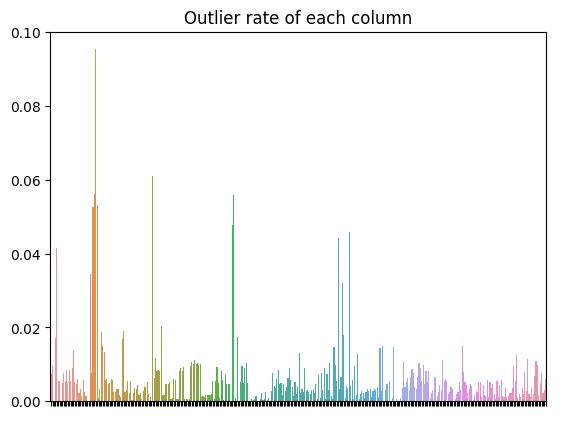
\includegraphics[height=6cm]{../img/outlier}
\caption{各列异常值率统计图}
\end{figure}

由上图可以看到,该数据集中整体异常值率均较高,超过0.003的属性列有相当多。我们猜测可能是因为金融数据中确实常有违背正态分布这一假设的数据,如各种涉及到金额的属性列大部分人可能均为0或者较低水平,而极少数人则动辄几十上百万,这点也能通过直接观察数据集得到验证。更进一步,我们还将各列及其对应异常值率数值进行了排序输出,前20个如下所示:
\begin{lstlisting}
[('CUST_GOLD_COMMON_FLAG', 0.09529417950470583),
 ('DEP_SA_FLAG', 0.06100566100566101),
 ('CUST_INTERNATIONAL_DIAMOND_FLAG', 0.05608777187724556),
 ('FUND_FLAG', 0.0558388979441611),
 ('CUST_STAD_PLATINUM_FLAG', 0.05317139001349527),
 ('CUST_INTERNATIONAL_SIL_FLAG', 0.05254044201412623),
 ('LOAN_FLAG', 0.047850395218816275),
 ('L6_CHANNEL_AUTO_IN_MAX_AMT', 0.045817340554182656),
 ('L3_CHANNEL_AUTO_IN_MAX_AMT', 0.044257496889075834),
 ('LAST_OPEN_TENURE_DAYS', 0.041372662425294006),
 ('CUST_INTERNATIONAL_GOLD_FLAG', 0.03450233976549766),
 ('L3_CHANNEL_AUTO_OUT_MAX_AMT', 0.03202762150130571),
 ('DEP_SA_FGCR_ACCOUNT_CNT', 0.020267451846399213),
 ('L6_CUST_DEBT_AVG_AMT', 0.018988029514345302),
 ('CUST_DEBT_AMT', 0.018823281981176717),
 ('L3_CHANNEL_AUTO_OUT_MIN_AMT', 0.017975007448691658),
 ('RELATED_REPAY_FLAG', 0.017361585782638415),
 ('bad_good', 0.017119722382880277),
 ('L3_CUST_DEBT_AVG_AMT', 0.01697600644969066),
 ('L6_CHANNEL_CTR_STAIN_AVGCNT', 0.01499553078500447)]
\end{lstlisting}

可以看到,异常值率最高的几列均为FLAG类属性列,而这些列一般来说都是对预测有帮助且很容易利用的;另外,预测目标列bad\_good的异常值率也达到了0.017左右,这也验证了前面的猜测。结合以上分析及信息,我们最终未根据异常值率对数据进行任何处理。

\subsection{处理后数据概览}
经过以上的全局预处理流程,处理后的训练集和测试集信息如下所示:(测试集没有bad\_good列)
\begin{lstlisting}
# 训练集
<class 'pandas.core.frame.DataFrame'>
RangeIndex: 285285 entries, 0 to 285284
Columns: 356 entries, OPEN_ORG_NUM to L6_CHANNEL_AUTO_DOUTTA_AVGCNT
dtypes: float64(260), int64(96)
memory usage: 774.9 MB
# 测试集
<class 'pandas.core.frame.DataFrame'>
RangeIndex: 189766 entries, 0 to 189765
Columns: 355 entries, OPEN_ORG_NUM to L6_CHANNEL_AUTO_DOUTTA_AVGCNT
dtypes: float64(259), int64(96)
memory usage: 514.0 MB
\end{lstlisting}

在处理后的训练集上,我们还计算了各列与目标列bad\_good的相关系数并绘图如下:

\begin{figure}[H]
\centering
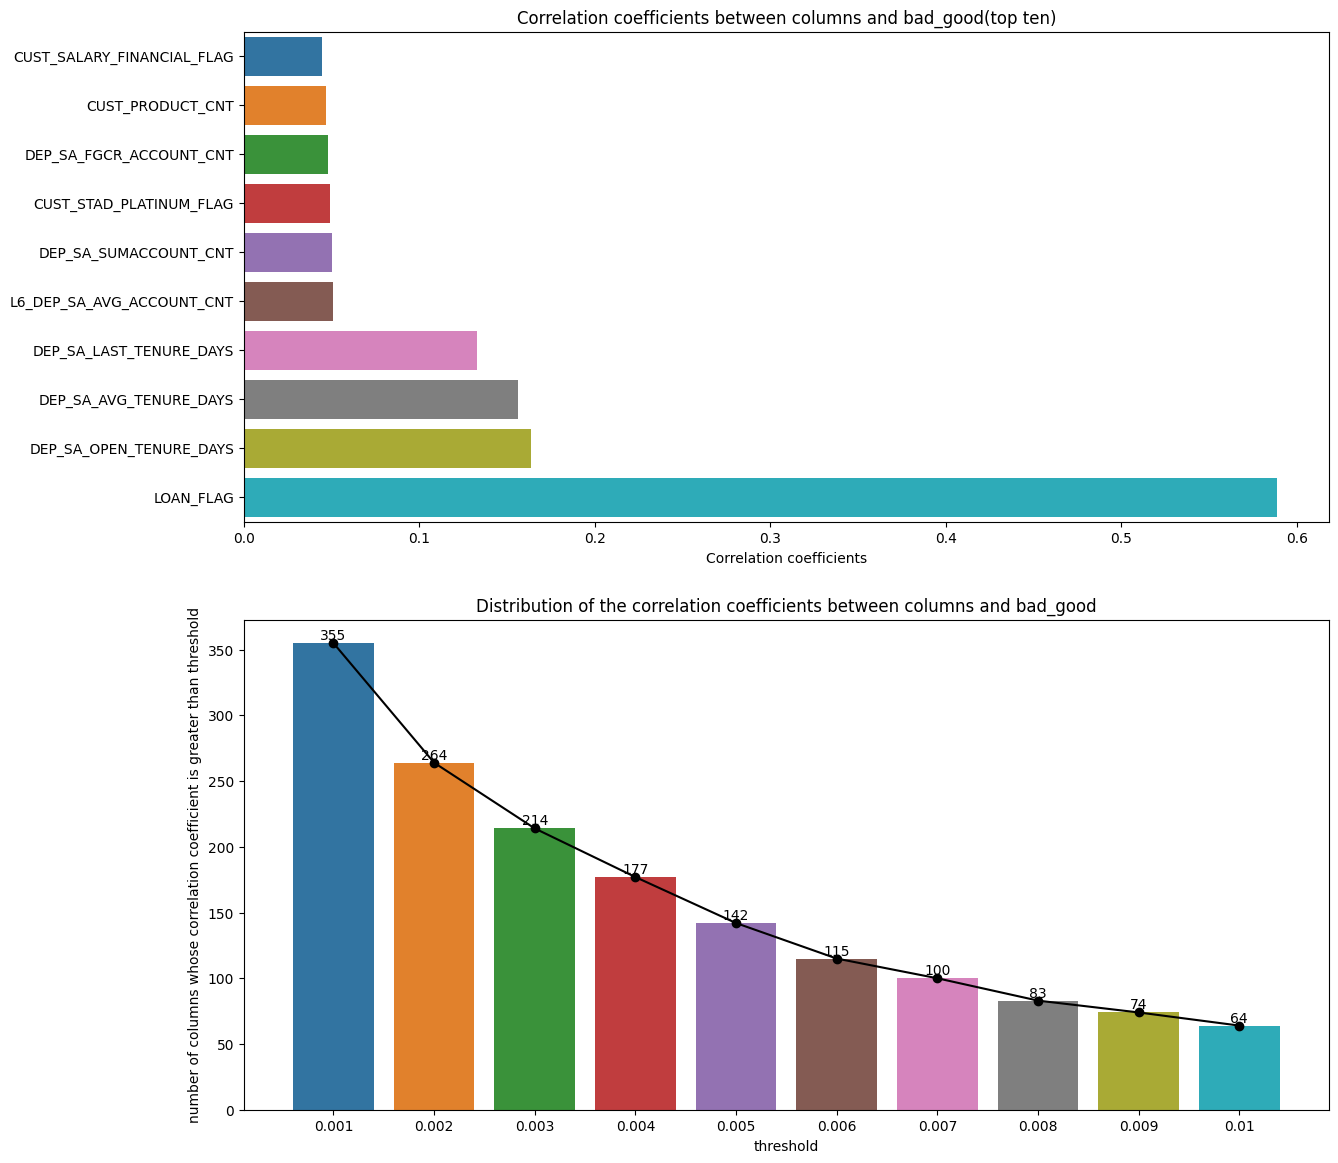
\includegraphics[height=12cm]{../img/corr}
\caption{与目标列相关系数最大的前10列以及相关系数在各阈值以上的属性列数量}
\end{figure}
可以看到,全局预处理后大部分属性列与bad\_good的相关性均较小,且在相关系数排序靠前的列中,不同列之间的差距很明显。以上绘图与分析结果将是后续各方法挑选特征的重要参考。

值得一提的是,由于后续各方法对数据的要求不同,如MLP方法训练前先归一化数据可以避免数值溢出、加快收敛,而Qwen1.5方法则不太需要,因此全局预处理过程仅针对各方法的共同需求进行数据处理,各方法在使用该数据时也可能会在此基础上进行各自的局部预处理。

 \setcounter{section}{3}
\section*{\centerline{三、多方法实施预测}}
\setcounter{subsection}{0}
\subsection{MLP(MLP.ipynb)}
看到赛题以及数据集之后,我们最先想到的方法也是最传统的方法就是前馈神经网络或者说多层感知机(MLP)了,我们计划先用该方法验证全局预处理的可行性。该方法最基础的结构就是输入层、若干隐藏层、输出层,使用非线性的激活函数,并通过反向传播来更新各个神经元的权重。已有研究证明,当中间隐藏层的神经元数量趋于无穷多时,多层感知机可以拟合任何非线性函数。

\subsubsection{局部预处理与数据集划分}
首先,在全局预处理后的数据集的基础上,为了避免数值溢出(金融数据取值跨度大),同时也可以加速收敛,我们先对所有属性列进行了最大-最小值归一化,将各列取值放缩到一致的范围。

其次,为避免不太相关的信息影响模型性能,同时还要保证模型有足够可以提取的特征,我们根据上文中的图2,选取了与目标列最相关的前100个属性列(即相关系数均大于0.007)进行训练。

然后,使用sklearn库函数中的train\_test\_split将挑选出的数据划分为训练集和验证集。考虑到总样本数为285285,故将验证集的比例设置为0.01。

\subsubsection{训练、验证与预测}
经测试,由于目标列正负样本极不平衡,当隐藏层的宽度或深度设置得较小时,预测结果很可能会显示全0,效果较差。经过多次调整后,选定隐藏层参数为(10, 10, 5),优化器为Adam,最大迭代次数扩大到500次,然后在训练集上进行训练。

模型训练完毕后,使用cross\_val\_score函数让模型在验证集上进行五折交叉验证并输出平均得分,作为测试集得分的一个估计;最后在测试集上进行预测,并将预测结果处理为竞赛网站上的提交格式即可。主要代码如下:
\begin{lstlisting}
# 选取前100列
data = df[cols[-100: ] + ['bad_good']].copy()
X_test = df_test[cols[-100: ]].copy()
train_data, valid_data = train_test_split(data, test_size=0.01)
X_train, y_train = train_data[cols[-100: ]], train_data['bad_good']
X_valid, y_valid = valid_data[cols[-100: ]], valid_data['bad_good']
# 训练与验证
model = MLPClassifier(hidden_layer_sizes=(10, 10, 5), solver='adam', max_iter=500)
model.fit(X_train, y_train)
score = cross_val_score(model, X_valid, y_valid, cv=5)
print(score.mean())
# 预测
y_pred = model.predict(X_test)
df_pred = pd.DataFrame({'bad_good': y_pred})
df_pred.insert(0, 'CUST_ID', df_submit['CUST_ID'])
\end{lstlisting}


\subsection{Qwen1.5}
考虑到用户逾期行为预测任务也是一个二分类任务,那么能不能像实验四一样利用预训练大模型在该任务上微调以使其达到较好的性能呢?于是我们在这方面也进行了尝试。

\subsubsection{实验环境}
本方法的实施全程在阿里云人工智能平台PAI的交互式建模(DSW)设备上进行,以下列出主要的配置信息:
\begin{itemize}
	\item 资源规格:ecs.gn7i-c8g1.2xlarge, 1 * NVIDIA A10(1 * 24 GB), 8 vCPU, 内存30GiB
	\item 环境信息: modelscope:1.15.0, pytorch2.3.0, tensorflow2.16.1, python3.10, cu121
\end{itemize}

\indent 考虑到使用的设备仅有一张24GB显存的A10显卡,我们选择了\textbf{Qwen1.5-1.8B-chat}模型,它是一个基于Transformer架构且只包含解码器的对话语言模型,并且已经经过了大量数据的预训练,拥有18亿左右的参数量。LoRA微调和推理过程则使用了SWIFT微调框架。

\subsubsection{数据集预处理(process\_Qwen1.5.ipynb)}
与实验四中文本分类不同,用户逾期行为预测任务的数据集是csv格式,且数据的组织形式也有很大差异,所以有必要在全局预处理的基础上针对chat模型再次处理数据。值得一提的是,本方法中我们无需再进行归一化操作,保持数据的原本面貌更有利于语言模型提取语义信息。

首先,考虑到设备资源以及模型最大输入长度的限制,我们难以在全部属性列和样本上进行微调。于是根据与目标列bad\_good的相关系数排序,我们选取了前\textbf{64}个(即相关系数大于0.01)属性列,并采样了\textbf{10000}个样本进行微调训练。

其次,要进行数据集的划分。为了不盲目在竞赛网站上提交,浪费提交次数,我们将全局预处理后的数据集按\textbf{9:1}的比例划分为训练集和验证集,这样便于我们把握模型在测试集上的大概性能水平。

接着,我们在构建输入到chat模型的数据集时,将每个样本的属性列名进行了替换。Qwen1.5毕竟是语言模型,我们认为如果单纯地把每个样本的属性列名及取值组合后作为文本输入,最终并不会有很好的效果,因为字段说明对于大模型“理解”我们的样本并进行分类应当是十分重要的。具体来说,就是根据“字段说明.xlsx”文件将每个样本的所有字段名进行逐一替换,每个样本的数据信息格式如下:

\begin{lstlisting}
<字段1说明>:<字段1取值>;<字段2说明>:<字段2取值>;...<字段64说明>:<字段64取值>;
\end{lstlisting}

然后,为了引导chat模型“理解”任务目标,加快微调过程收敛速度,输出任务需要的、便于后续评估计算的输出,需要进行良好的prompt设计。经过多次调整与精简,我们的prompt格式如下所示:

\begin{lstlisting}
"以下为某银行真实信贷用户信息:\n<样本数据信息>\n请根据这些信息判断该用户信贷是否逾期,仅输出0或1:"
\end{lstlisting}

最后,参考swift框架对自定义数据集格式的规定,我采用了单轮对话格式的输入(即query+response)。考虑到是chat模型,response中需标注为字符串类型的0或1。将预处理完成后的训练集、验证集、测试集各自保存。以下为验证集中一个样本处理后的内容:
\begin{lstlisting}
{"query": "以下为某银行真实信贷用户信息:\n本期自助设备借方交易笔数:0.0;私人银行理财金额:0.0;6个月银保通月日均金额:0.0;持有基金标志:1.0;六个月月平均持有本币余额:8437.9233333;本月活期存款月日均余额:10518.566;......三个月月平均持有本币余额:16085.91;其它转入三个月内最大交易金额:1377363.57;最近三个月活期存款月日均余额:5268.5274839;......持有外币账户数量:2.0;是否标准白金卡:0.0;当月存款账户总数:4.0;六个月月均存款账户总数:4.0;活期存款最近开户距今月份:774.0;活期存款平均开户时长:858.0;活期存款最早开户日期距今月份:956.0;个贷标识:0.0;\n请根据这些信息判断该用户信贷是否逾期,仅输出0或1:", "response": "0"}
\end{lstlisting}

\subsubsection{模型训练、验证与测试}

我们采取编写运行sh脚本的方式对Qwen1.5-1.8B-chat模型进行训练(微调)、验证以及测试(推理)。其中,sft.sh脚本同时进行微调与验证,infer.sh脚本则在测试集上进行推理,将推理结果提取并调整为竞赛要求的提交格式的代码则附在了process\_Qwen1.5.ipynb文件最后。

\textbf{sft.sh脚本内容如下:}
\begin{lstlisting}
# Experimental environment: A10
# 20GB GPU memory
PYTHONPATH=../../.. \
CUDA_VISIBLE_DEVICES=0 \
python llm_sft.py \
    --model_type qwen1half-1_8b-chat \
    --model_id_or_path /mnt/workspace/Qwen1.5-1.8B-Chat \
    --sft_type lora \
    --template_type AUTO \
    --dtype AUTO \
    --output_dir /mnt/workspace/output \
    --dataset /mnt/workspace/data/train_dataset.jsonl \
    --val_dataset /mnt/workspace/data/valid_dataset.jsonl \
    --train_dataset_sample -1 \
    --num_train_epochs 1 \
    --max_length 2048 \
    --check_dataset_strategy none \
    --gradient_checkpointing true \
    --batch_size 1 \
    --weight_decay 0.1 \
    --learning_rate 1e-4 \
    --gradient_accumulation_steps 16 \
    --max_grad_norm 0.5 \
    --warmup_ratio 0.03 \
    --eval_steps 50 \
    --save_only_model false \
    --save_total_limit 2 \
    --logging_steps 10 \
    --lora_rank 8 \
    --lora_alpha 16 \
    --lora_dropout_p 0.05 \
\end{lstlisting}

其中,model\_id\_or\_path为本地预训练模型路径,sft\_type lora表示启用LoRA微调方法,output\_dir表示微调过程中所有输出(包括checkpoint、微调参数设置、loss/acc等各种图像)的保存路径,dataset和val\_dataset分别指定了预处理后的训练集和验证集,warmup\_ratio表示warmup占用总的训练steps的比例,eval\_steps表示每隔多少steps用验证集评估一次(考虑到时间原因,设为50),save\_total\_limit 2表示最多保存两个checkpoints(即当前的和上一个)。
LoRA参数方面,lora\_dropout\_p表示随机drop的概率,防止过拟合;另外考虑到微调数据集较大,为控制微调时间,我们将lora\_rank设置为8,lora\_alpha则保持为前者的两倍。

运行上述脚本需要依次执行以下代码:
\begin{lstlisting}
# 添加可执行权限
cd /mnt/workspace/swift/examples/pytorch/llm/scripts/qwen1half_1.8b_chat/lora
chmod +x sft.sh
# 运行脚本
cd /mnt/workspace/swift/examples/pytorch/llm
./scripts/qwen1half_1.8b_chat/lora/sft.sh
\end{lstlisting}

\textbf{infer.sh脚本内容如下:}
\begin{lstlisting}
# 直接推理
CUDA_VISIBLE_DEVICES=0 swift infer \
    --ckpt_dir '/mnt/workspace/output/qwen1half-1_8b-chat/v0-20240629-164430/checkpoint-562' \
    --load_dataset_config true \
    --val_dataset /mnt/workspace/data/test_dataset.jsonl \
    --show_dataset_sample -1
\end{lstlisting}

其中,ckpt\_dir表示微调阶段保存的checkpoint(一般选择最后一个)路径,从该路径下可读取微调后模型配置信息,val\_dataset使用了预处理后的测试集,show\_dataset\_sample -1则表示将数据集中数据全部进行推理并展示。运行脚本的方法与前述类似。

上述脚本会输出测试集对应的包含query、response、label等字段的推理结果jsonl文件到所使用的checkpoint文件夹下,我们还需要对推理结果文件进行进一步处理使其符合可以在竞赛网站上提交的格式,代码如下:
\begin{lstlisting}
df_result = pd.read_json('output/qwen1half-1_8b-chat/v0-20240629-164430/checkpoint-562/infer_result/20240629-175456.jsonl', lines=True)
df_pred = pd.DataFrame({'bad_good': df_result['response']})
df_pred.insert(0, 'CUST_ID', df_submit['CUST_ID'])
df_pred.to_csv('result_Qwen1.5.csv', mode='w', index=False)
\end{lstlisting}

\setcounter{section}{4}
\section*{\centerline{四、实验结果对比与分析}}
\setcounter{subsection}{0}
\subsection{MLP}
MLP方法训练得到的模型在验证集上的五折交叉验证acc为0.9887872922235538,这说明模型性能已经达到了比较好的水平;然后将MLP模型在测试集上预测得到的result\_MLP.csv文件提交到竞赛网站上,最终得分\textbf{0.99921783352}超出了我们的预期。这也说明我们的预处理方法是具有相当的可行性的,MLP方法尽管较为传统但对数据分类任务也具有着相当强的拟合能力。

\subsection{Qwen1.5}

\begin{figure}[H]
\centering
\begin{minipage}[b]{0.49\textwidth}
\centering
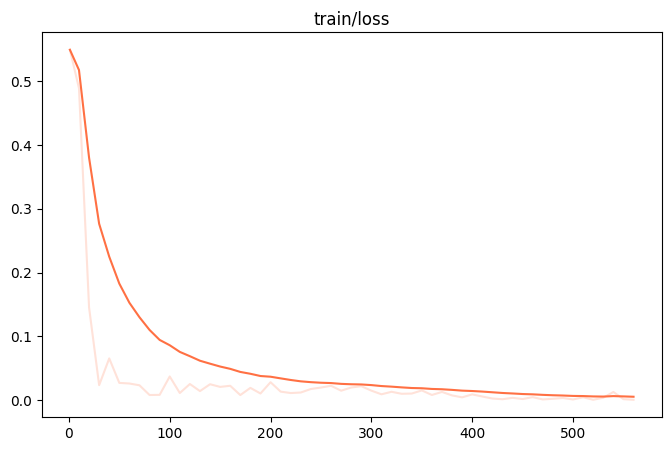
\includegraphics[height=4cm]{../img/train_loss}
\end{minipage}
\begin{minipage}[b]{0.49\textwidth}
\centering
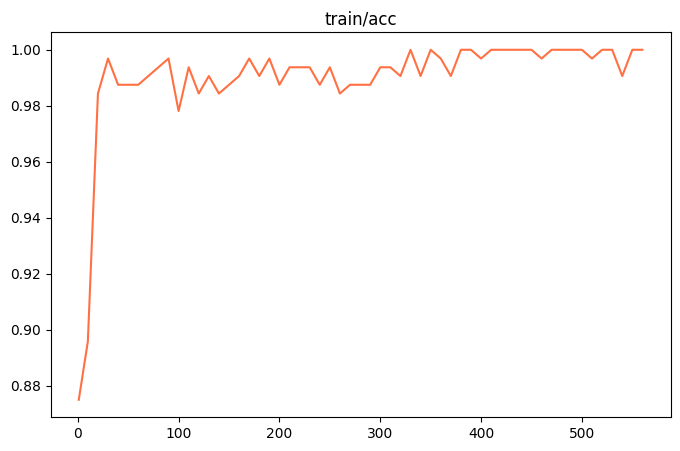
\includegraphics[height=4cm]{../img/train_acc}
\end{minipage}
\caption{微调过程训练集上模型表现}
\end{figure}

\begin{figure}[H]
\centering
\begin{minipage}[b]{0.49\textwidth}
\centering
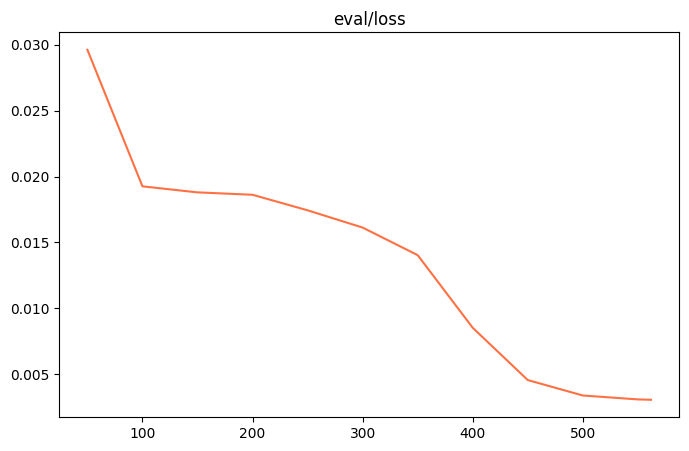
\includegraphics[height=4cm]{../img/eval_loss}
\end{minipage}
\begin{minipage}[b]{0.49\textwidth}
\centering
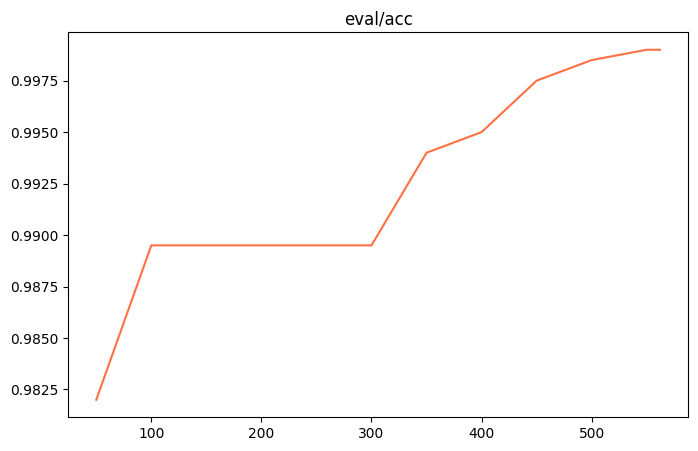
\includegraphics[height=4cm]{../img/eval_acc}
\end{minipage}
\caption{微调过程验证集上模型表现}
\end{figure}

观察上述结果可以看到,将用户逾期行为预测任务部署在预训练模型上微调的方法是可行的。不仅训练集上的loss稳步下降,acc快速上升并保持较高水平,而且在验证集上的性能表现也较为优秀。

但将Qwen1.5方法流程执行完后得到的result\_Qwen1.5.csv文件提交到竞赛网站上后,\textbf{0.95179323211}的得分却低于我们对大模型性能的预期。经过分析我们认为可能有以下几点原因:一是特征选取数量,目前的64个特征在进行列名替换后最长的一个样本长度达到了1279,为此我们设置了最长输入长度(max\_length)为2048,特征较少可能会丢失信息,特征较多则会造成输入过于冗长,需要在二者间进行权衡;二是样本采样方法,由于时间原因我们只随机采样了1w条样本(微调耗时约50分钟),但由于数据集正负样本数量极不均衡,采样较少可能会丢失信息,可以考虑更平衡的采样方法或更多的采样数量;三是文本化程度,我们在实验中已经进行了字段说明的替换,但每个字段的取值仍是数据形式的,如果将两者组合式地转化为文本,如“是否国际金卡:0.0”进一步转化为“不是国际金卡账户”,或者再进一步使用更具描述性的语言介绍每个用户的信息等等,性能是否会提升还有待探究。

但遗憾的是,由于测试集规模相当大,每次在测试集上推理时都要耗费巨量的时间(我们上述的参数设置推理了5小时左右),所以难以多次调参来深入探究。

\setcounter{section}{5}
\section*{\centerline{五、组内分工}}
\setcounter{subsection}{0}

\end{document}